\documentclass[11pt,titlepage]{book}
\usepackage{Preamble}

\begin{document}

\begin{titlepage}
    \newgeometry{margin=3cm}
	\centering
%    \includegraphics[width=0.8\linewidth]{BIT.png}\\[0.25cm] 	% University Logo
    \textsc{\LARGE Jianting's Lecture Review Notes}\\ \vspace{\fill}
    \textbf{\textsc{\fontsize{20}{20}\selectfont 最优化方法\\ Optimization Methods}}\\ \vspace{\fill}
    \medskip
    \textsc{2020 Fall}\\
    \medskip
    \textsc{Instructor : 李庆娜}\\
    \medskip
    \textsc{Textbook : 最优化方法}\\
    \bigskip
	\textsc{Review for Optimization Method}\\[0.4cm]
	\rule{\linewidth}{0.2 mm} \\[0.5 cm]
	Jianting Feng\\
	\today\\
	BEIJING INSTITUTE OF TECHNOLOGY
\end{titlepage}
\restoregeometry

\frontmatter 
\chapter{前言}
这是笔者于2020年秋季学期于北京理工大学良乡校区学习最优化方法课程时的笔记总结,由于一些众所周知的原因,该笔记参考的主要书目并不为课程所指定的教材,而是:刘浩洋, 户将, 李勇锋,文再文,最优化:建模、算法与理论, 高教出版社, 书号978-7-04-055035-1
H. Liu, J. Hu, Y. Li, Z. Wen, Optimization: Model, Algorithm and Theory (in Chinese)
详情可参考\href{http://bicmr.pku.edu.cn/~wenzw/optbook.html}{文再文老师的主页}。截止笔者完成该份笔记之前,本书还处于\textbf{即将出版}的状态。\par
另外一本个人觉得比较好的参考资料为Algorithms for Optimization
By Mykel J. Kochenderfer and Tim A. Wheeler。本书由MIT出版社出版,可以在MIT Press的\href{https://mitpress.mit.edu/books/algorithms-optimization}{官网}购买该书并下载相应代码与Slides(文老师的教材也可在相应网站下载代码)。
\par
顺便吐槽一句,这课讲的东西真的不是最优化,证明都跟没讲一样,倒是幻灯片上有不少算例,这就算一个将数值优化方法的课吧。最后,LQNYYDS!
\par
\bigskip
Jianting Feng\\
2020年11月\\
于北京理工大学
\newpage
\tableofcontents
\newpage
\thispagestyle{numberonly}
\mainmatter 
\chapter{预备知识 Preliminary}
\section{多元微积分}
\subsection{多元函数的Taylor展开}
\begin{equation}
	f(\bm{x}_0+\bm{p}) = f(\bm{x}_0)+\nabla f(\bm{x_0})^T\bm{p} + o(||\bm{p}||)
\end{equation}
\begin{equation}
	f(\bm{x}_0+\bm{p}) = f(\bm{x}_0)+\nabla f(\bm{x_0})^T\bm{p} + \frac{1}{2}\bm{p}^Tf(\bm{x}_0)\bm{p} + o(||\bm{p}||)^2
\end{equation}
若$f(\bm{x}) = \bm{b}^T\bm{x}$,则有
\begin{equation}
	\nabla f(\bm{x}) = \bm{b},\quad \nabla^2 f(\bm{x}) = 0_{n\times n}
\end{equation}
若$f(\bm{x}) = \frac{1}{2}\bm{x}^TQ\bm{x}$,且$Q$为对称方阵,则有
\begin{equation}
	\nabla f(\bm{x}) = Q\bm{b},\quad \nabla^2 f(\bm{x}) = Q
\end{equation}
\section{线性空间中的范数}
\begin{definition}
	在$n$维线性空间$\mathbb{R}^n$中,定义
	\begin{equation*}
			||\cdot||:\mathbb{R}^n \rightarrow \mathbb{R}
	\end{equation*}
	满足下述三条公理:
	\begin{enumerate}
		\item (正定性)$\forall \bm{x}\in \mathbb{R}^n$,有$||\bm{x}||\geq 0$,且$||\bm{x}||= 0$当且仅当$\bm{x} = \bm{0}$;
		\item $\forall \bm{x}\in \mathbb{R}^n$及$\alpha \in \mathbb{R}$,有$||\alpha \bm{x}|| = |\alpha|||\bm{x}||$;
		\item $\forall \bm{x}, \bm{y}\in \mathbb{R}^n$,有$||\bm{x}+\bm{y}||\leq ||\bm{x}||+ ||\bm{y}||$
	\end{enumerate}
	则称$||\cdot||$为$\mathbb{R}^n$上的一个范数(norm)。
\end{definition}
\begin{example}
	常用的范数有如下几个:
	\begin{enumerate}
		\item $2$-范数:$||\bm{x}||_2 = (\sum\limits_{i=1}^n x_i^2)^{\frac{1}{2}}$
		\item $\infty$-范数:$||\bm{x}||_\infty = \max\limits_{1\leq i\leq n}|x_i|$
		\item $1$-范数:$||\bm{x}||_\infty = \sum\limits_{i=1}^n|x_i|$
	\end{enumerate}
\end{example}
\section{凸集与凸函数}
\begin{definition}
	设$D\subseteq \mathbb{R}^n$,若对于任意的$\lambda\in [0, 1]$,都有
	\begin{equation*}
		\lambda x + (1-\lambda )y \in D,
	\end{equation*}
	则称$D$为\textbf{凸集}。
	称$\lambda x + (1-\lambda )y$为凸组合。
\end{definition}
\begin{note}
	用数学归纳法,容易证明对于任意有限个元素的凸组合仍满足上述性质。
\end{note}
\subsection{几个重要且常见的凸集}
\subsubsection{超平面与半空间}
对于任意非零向量$a$,我们称形如$\{x\mid a^Tx = b\}$的集合为\textbf{超平面},形如$\{x\mid a^Tx \leq b\}$的集合为\textbf{半空间}。
\subsubsection{球、椭球、锥}
\begin{definition}
	设$||\cdot||$为一个范数,定义
	\begin{equation*}
		B(x_c, r) = \{x\mid ||x-x_c||\leq r\}
	\end{equation*}
	为半径为$r$,中心为$x_c$的\textbf{球}。
\end{definition}
\begin{definition}
	形如
	\begin{equation*}
		\{x\mid (x-x_c)^TP^{-1}(x-x_c)\leq 1\}
	\end{equation*}
	中心为$x_c$的\textbf{椭球},其中$P\in\mathcal{S}_{++}^n$(即$P$对称正定)。
\end{definition}
\begin{definition}
	称集合
	\begin{equation*}
		\{(x, t)\mid ||x||\leq t\}
	\end{equation*}
	为\textbf{范数锥},Euclid范数锥也称\textbf{二次锥}。
\end{definition}
更多与锥(cone)相关的内容,请参考\ref{cone}

\begin{definition}[凸函数]
	设$f(\bm(x))$为适当函数,如果$f$的定义域$D$为凸集,且满足
	\begin{equation*}
		f(\lambda x + (1-\lambda )y)\leq \lambda f(x) + (1-\lambda) f(y)
	\end{equation*}
	对于所有$x,y\in D$与$0\leq \lambda \leq 1$都成立,则称$f$是\textbf{凸函数}。
\end{definition}
\begin{definition}[严格凸函数]
	设$f(\bm(x))$为适当函数,如果$f$的定义域$D$为凸集,且满足
	\begin{equation*}
		f(\lambda x + (1-\lambda )y)< \lambda f(x) + (1-\lambda) f(y)
	\end{equation*}
	对于所有$x,y\in D$与$0< \lambda < 1$都成立,则称$f$是\textbf{严格凸函数}。
\end{definition}
\begin{theorem}[凸函数的判定定理]
	$f(x)$是定义在凸集$D\subset \mathbb{R}^n$上的(严格)凸函数,则对于任意$x, y\in D$,令
	\begin{equation*}
		\phi(t) = f(tx + (1-t)y), \quad t\in [0, 1]
	\end{equation*}
	$\phi(t)$为$[0, 1]$上的(严格)凸函数。
\end{theorem}
\begin{note}
	事实上,上面定理的说的是,凸函数的一个最基本的判定方式是:先将其限制在任意直线上,然后判断对应的一维函数是否是凸的。
\end{note}
对于可微函数,我们判断其是否为凸函数还可以根据它的导数信息来判断
\begin{theorem}[一阶条件]
	对于定义在凸集$D\subset \mathbb{R}^n$上的可微函数$f$,$f$是凸函数当且仅当下式成立
	\begin{equation*}
		f(y)\geq f(x) +\nabla f(x)^T(y-x)\quad \forall x, y\in D.
	\end{equation*}
\end{theorem}
\begin{theorem}[二阶条件]
	对于定义在凸集$D\subset \mathbb{R}^n$上的二阶连续可微函数$f$,$f$是凸函数当且仅当下式成立
	\begin{equation*}
		\nabla^2 f(x)\succeq 0\quad \forall x\in D.
	\end{equation*}
	如果$\nabla^2 f(x)\succ 0\quad \forall x\in D$,则$f$是严格凸函数。
\end{theorem}
\begin{definition}[水平集]
设函数$f(x)$定义在$D$上,
	\begin{equation*}
		D_\alpha := \{x\mid x\in D, f(x)\leq \alpha\}
	\end{equation*}
	称为$f(x)$的\textbf{水平集}。
\end{definition}
由水平集的定义及凸函数的判定性质,立即有
\begin{theorem}
	凸集上的凸函数的水平集为凸集,即
	设凸函数$f(x)$定义在凸集$D\subset \mathbb{R}^n$上,则
	\begin{equation*}
		D_\alpha = \{x\mid x\in D, f(x)\leq \alpha\}
	\end{equation*}
	为凸集。
\end{theorem}
\section{凸规划}
设凸函数$f(x)$定义在凸集$D\subset \mathbb{R}^n$上,则下列规划问题
\begin{equation*}
	\begin{split}
		&\min f(x)\\
		&s.t.\begin{cases}
			g_i(x)\geq 0,\quad i = 1,2,\cdots, m\\
			h_j(x) = 0, j=1,2,\cdots, l
		\end{cases}
	\end{split}
\end{equation*}
若$g_i(x)$为凸函数,$h_j(x)$为线性函数,则上述问题称为\textbf{凸规划}。
\section{收敛速度}
\begin{definition}
	设序列$\{\bm{x}_k\}$收敛于$\bm{x^*}$,且有
	\begin{equation*}
		\lim\limits_{k\to \infty}\frac{||\bm{x}_{k+1} - \bm{x}^*||}{||\bm{x}_{k} - \bm{x}^*||} = \beta
	\end{equation*}
	\begin{enumerate}
		\item 若$\beta = 1$,则称该序列\textbf{次线性收敛}
		\item 若$0<\beta<1$,则称该序列\textbf{线性收敛},$\beta$被称为\textbf{收敛比}
		\item 若$\beta = 0$,则称该序列\textbf{超线性收敛}
	\end{enumerate}
\end{definition}
\begin{definition}
	设序列$\{\bm{x}_k\}$收敛于$\bm{x^*}$,若对于某个实数$p\geq 1$,有
	\begin{equation*}
		\lim\limits_{k\to \infty}\frac{||\bm{x}_{k+1} - \bm{x}^*||}{||\bm{x}_{k} - \bm{x}^*||^p} = \beta,\quad 0<\beta < +\infty
	\end{equation*}
	则称该序列为$p$阶收敛的.
\end{definition}
\chapter{线性规划 Linear Programming}

\chapter{无约束优化问题 Unconstrained Optimization}
本节考虑如下的无约束优化问题:
\begin{equation}\label{ucp}
	\min\limits_{x\in\mathbb{R}^n} f(x),
\end{equation}
其中$f(x): \mathbb{R}^n\to\mathbb{R}$
\section{线搜索方法}
线搜索算法的数学表述为:给定当前点$x^k$,首先通过某种算法(稍后会涉及)选取\textbf{下降方向}$d^k$,确定\textbf{步长}$\alpha_k>0$,则下一步的迭代点可以写作
\begin{equation}\label{iter}
	x^{k+1} = x^k + \alpha_k d^k
\end{equation}
$d^k$是下降方向的要求为$(d^k)^T\nabla f(x^k)$,即要求了沿该方向函数值$f$会减小。线搜索回答了如何选择一个合适的步长$\alpha_k$.\par
实际上这是一个一维的优化问题,我们构造辅助函数
\begin{equation*}
	\phi(\alpha) = f(x^k+\alpha d^k)
\end{equation*}
显然,这是将$f(x)$限制在$\{x^k+\alpha d^k: \alpha > 0\}$一个一维区域上.线搜索的目的实际上是选取合适的$\alpha_k$使得$\phi(\alpha_k)$足够小,于是我们有两种想法:找到使函数值在该方向上的最小值或找到一个能够使函数值下降的步长(不需要下降到最小值),分别称为\textbf{精确线搜索算法}与\textbf{非精确线搜索算法}.
\subsection{精确线搜索算法}
正如上面所讨论的相同, 我们是求解如下的问题
\begin{equation*}
	\alpha_k = \arg \min\limits_{\alpha>0} \phi(\alpha),
\end{equation*}
即$\alpha_k$为最佳步长, 这实际上可能需要极大的计算量(针对光滑函数可以想象为求导函数的根,详情参见数值计算方法中求解非线性方程),所以我们在实际应用中很少使用这种方法,我们仅需要$\phi(\alpha_k)$满足一些不等式性质,这样产生的算法就是我们下面要介绍的\textbf{非精确搜索算法}
\subsection{Armijo准则}
首先,我们引入一个较为常用的线搜索准则,它保证了每一步迭代充分下降.
\begin{definition}[Armijo准则]
	设$d^k$为点$x^k$处的下降方向, 若
	\begin{equation*}\label{armijo}
		f(x^k+\alpha d^k)\leq f(x^k)+ c_1\alpha \nabla f(x^k)^Td^k,
	\end{equation*}
	则称步长$\alpha$满足\textbf{Armijo准则},其中$c_1\in (0, 1)$是一个预先给定的常数.
\end{definition}
Armijo准则的几何意义也是很明显的,参见下图
\begin{figure}[h!]
\caption{Armijo准则}
\centering
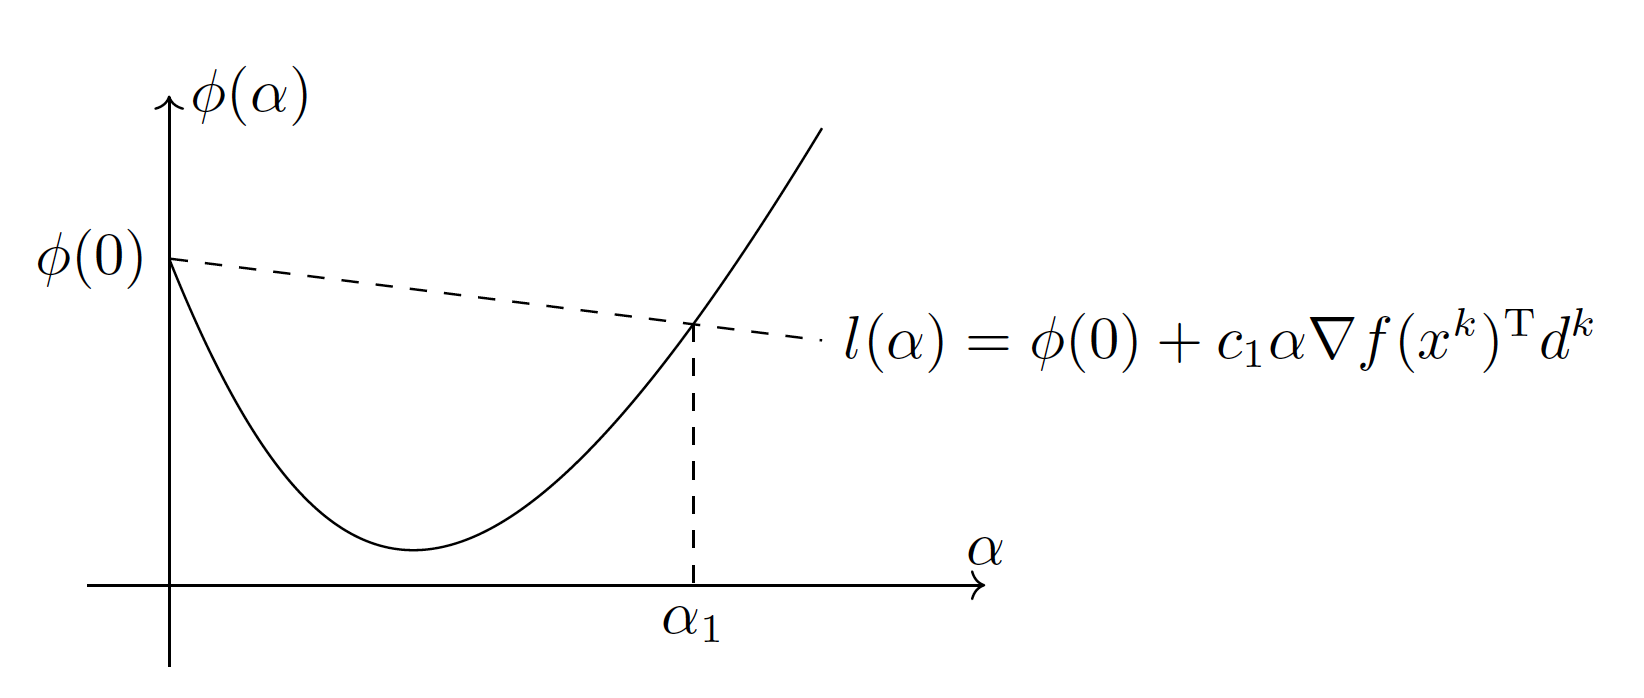
\includegraphics[width=0.8\textwidth]{img/armijo.png}
\end{figure}
它的含义是指点$(\alpha, \phi(\alpha))$必须在直线
\begin{equation*}
	l(\alpha) = \phi(0) +c_1\alpha \nabla f(x^k)^Td^k
\end{equation*}
的下方,由于$d^k$选取的是下降方向, 于是$\nabla f(x^k)^Td^k<0$,该直线的斜率一定为负.通常应用中取$c_1$足够小,这样使得Armijo条件非常容易满足,但是,如果选取的步长太小,那么迭代的点可能固定不变.\par
在实际使用过程中,我们常常将Armijo算法与\textbf{回退法}一同使用.给定初值$\hat{\alpha}$,回退法通过不断以指数方式缩小来试探步长,找到的第一个满足Armijo准则的点.
\begin{algorithm}[H]
%\footnotesize%字体大小
\caption{线搜索回退法}%首行显示算法名称
\begin{algorithmic}[1]%行编号,从Input, Output后面开始
%输入Input
\State 选择初始步长$\hat{\alpha}$,参数$\gamma, c\in (0, 1)$.初始化$\alpha\leftarrow \hat{\alpha}$.
\While{$f(x^k+\alpha d^k) > f(x^k)+ c_1\alpha \nabla f(x^k)^Td^k,$}
\State 令$\alpha \leftarrow \gamma \alpha$
\EndWhile
\State 输出$\hat{\alpha} = \alpha$
\end{algorithmic}  
\end{algorithm}
\subsection{Wolfe-Powell准则}
Wolfe-Powell准则也叫做Wolfe准则或Armijo-Wolfe准则.
\begin{definition}[Wolfe准则]
	设$d^k$是点$x^k$处的下降方向,若
	\begin{equation}\label{wolfe}
		\begin{split}
			&f(x^k+\alpha d^k)\leq f(x^k) + c_1\alpha \nabla f(x^k)^T d^k,\\
			&\nabla f(x^k + \alpha d^k)^T d^k \geq c_2 \nabla f(x^k)^Td^k,
		\end{split}
	\end{equation}
	则称步长$\alpha$满足\textbf{Wolfe准则},其中$c_1, c_2\in (0, 1)$为给定常数且有$c_1<c_2$.
\end{definition}
准则中第一个不等式即为Armijo准则,而第二个不等式为Wolfe准则的要求.注意到$\nabla f(x^k+\alpha d^k)^Td^k$恰好为$\phi(\alpha)$的导数,Wolfe准则实际要求$\phi(\alpha)$在$\alpha$处的切线斜率不能小于$\phi'(0)$的$c_2$倍.如图所示,在$[\alpha_1, \alpha_2]$中的点均满足Wolfe准则,并且在极小值点$\alpha^*$处有$\phi(\alpha^*) = \nabla f(x^k+\alpha^*d^k)^Td^k = 0$,于是$\alpha^*$永远满足第二个不等式, 只需选择较小的$c_1$满足第一个不等式即可。
\begin{figure}[h!]
\caption{Wolfe准则}
\centering
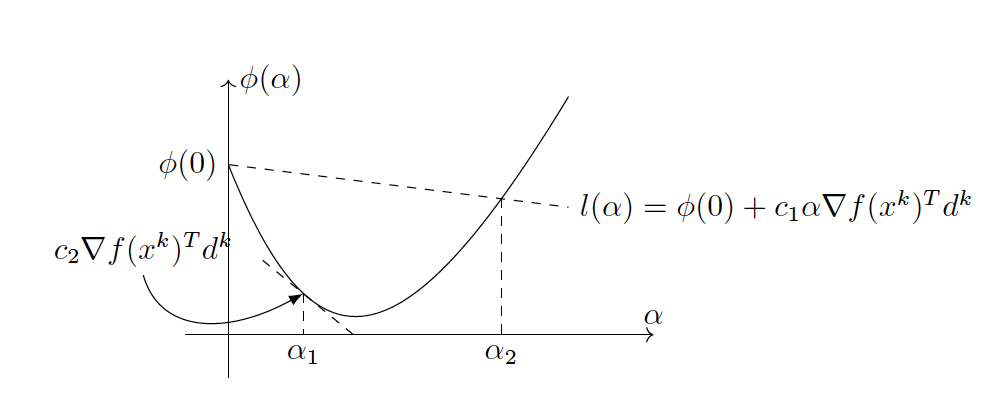
\includegraphics[width=0.8\textwidth]{img/wolfe.png}
\end{figure}
\subsection{线搜索法的收敛性分析}
\begin{theorem}[Zoutendijk]
	考虑一般的迭代格式\eqref{iter}.其中$d^k$是搜索发现, $\alpha_k$是步长, 且在迭代的过程中满足Wolfe准则. 假设目标函数$f$下有界、连续可微且梯度$\nabla f$ Lipschitz连续,即
	\begin{equation*}
		||\nabla f(x) - \nabla f(y)||\leq L||x-y||,\quad \forall x, y \in \mathbb{R}^n,
	\end{equation*}
	那么我们有
	\begin{equation*}
		\sum\limits_{k=0}^\infty \cos^2\theta_k ||\nabla f(x^k)||^2\leq +\infty
	\end{equation*}
	其中$\cos\theta_k$为负梯度$-\nabla f(x^k)$和下降方向$d^k$夹角的余弦, 即
	\begin{equation*}
		\cos\theta_k = \frac{-\nabla f(x^k)^Td^k}{||\nabla f(x^k)||||d^k||
}
	\end{equation*}
\end{theorem}
这个定理的证明是某老师喜欢考的,所以我们在此仔细加以讨论
\begin{proof}
	由Wolfe准则的第二个不等式,我们有
	\begin{equation*}
		(\nabla f(x^{k+1}) - \nabla f(x^k))^T d^k \geq (c_2 - 1)\nabla f(x^k)^Td^k.
	\end{equation*}
	有Cauchy-Schwarz不等式与Lipschitz条件
	\begin{equation*}
		\begin{split}
			(\nabla f(x^{k+1}) - \nabla f(x^k))^T d^k &\leq ||\nabla f(x^{k+1}) - \nabla f(x^k)||\ ||d^k||\\
			& \leq L||x^{k+1}-x^k||\ ||d^k||\\
			& \leq \alpha_k L ||d^k||^2.
		\end{split}
	\end{equation*}
	结合上面俩式,有
\begin{equation*}
	(c_2 - 1)\nabla f(x^k)^Td^k \leq \alpha_k L ||d^k||^2
\end{equation*}
即步长$\alpha_k$满足
\begin{equation*}
	\alpha_k \geq \frac{(c_2 - 1)\nabla f(x^k)^Td^k}{L ||d^k||^2}
\end{equation*}
将此式代入Wolfe准则的第一个不等式,得到
\begin{equation*}
	\begin{split}
		f(x^{k+1}) &\leq f(x^k) + c_1 \frac{(c_2 - 1)\nabla f(x^k)^Td^k}{L ||d^k||^2} \nabla f(x^k)^T d^k\\
		& = f(x^k)+\frac{c_1(c_2-1)}{L}\frac{(\nabla f(x^k)^T d^k)^2}{||d^k||^2}\\
		& = f(x^k)-\frac{c_1(1-c_2)}{L}\cos^2\theta_k ||\nabla f(x^k)||^2.
	\end{split}
\end{equation*}
这显然是一个递推的不等式, 右侧关于$k$递推(从$k$到$0$),得到
\begin{equation*}
	f(x^{k+1})\leq f(x^0)-\frac{c_1(1-c_2)}{L}\sum\limits_{j=0}^k\cos^2\theta_j ||\nabla f(x^j)||^2
\end{equation*}
由于$f$是下有界且下降的(Wolfe准则保证了严格下降性),同时由于$0<c_1<c_2<1$,有$c_1(1-x_2)>0$,于是我们得到了
\begin{equation*}
	\sum\limits_{j=0}^k\cos^2\theta_j ||\nabla f(x^j)||^2 < +\infty
\end{equation*}
令$k\to\infty$,得到我们所需要的
\begin{equation}\label{Zoutendijk}
	\sum\limits_{j=0}^\infty \cos^2\theta_j ||\nabla f(x^j)||^2 < +\infty
\end{equation}
\end{proof}
该定理指出了在满足Wolfe准则,对梯度Lipschitz连续且下有界的函数总能得到\eqref{Zoutendijk}条件成立.Zoutendijk定理实际上刻画了线搜索准则的性质, 配合一定的下降方向$d^k$选取方式, 我们能够得到线搜索最基本的收敛性.
\begin{theorem}[线搜索算法的收敛性]
	对于迭代格式\eqref{iter},设$\theta_k$为每一步迭代过程中下降方向$d^k$与负梯度方向$-\nabla f(x^k)$的夹角, 并且假设对于任意的$k$,都存在常数$\gamma$使得
	\begin{equation*}
		\theta_k < \frac{\pi}{2} - \gamma
	\end{equation*}
	严格成立,则在\eqref{Zoutendijk}条件成立的前提下, 我们能得到算法一定是收敛的,即
	\begin{equation*}
		\lim\limits_{k\to\infty} \nabla f(x^k) = 0.
	\end{equation*}
\end{theorem}
\begin{proof}
	直接证明较为困难,我们考虑反证法, 假设存在子列$\{k_l\}$和正常数$\delta > 0 $,使得结论不成立,即
	\begin{equation*}
		||\nabla f(x^{k_l})||\geq \delta,\quad l = 1, 2, \cdots,
	\end{equation*}
	根据$\theta_k$的假设,对任意$k$,有
	\begin{equation*}
		\cos\theta_k >\sin\gamma >0.
	\end{equation*}
	于是
	\begin{equation*}
		\begin{split}
			\sum\limits_{k=0}^\infty \cos^2\theta_k ||\nabla f(x^k)||^2  &\geq \sum\limits_{l=1}^\infty \cos^2\theta_{k_l} ||\nabla f(x^{k_l})||^2 \\
			&\geq \sum\limits_{l=1}^\infty (\sin^2\gamma)\cdot \delta^2\rightarrow +\infty
		\end{split}
	\end{equation*}
	这与\eqref{Zoutendijk}矛盾,因此一定有
	\begin{equation*}
		\lim\limits_{k\to\infty} \nabla f(x^k) = 0.
	\end{equation*}
\end{proof}
\begin{note}
	这个推论的几何意义是显然的, 如果下降方向$d^k$与梯度方向正交的话,根据Taylor公式的一阶近似, 函数值$f(x^k)$几乎不发生改变,因此我们在后面求解下降方向时,总是要求它与梯度的垂直方向的夹角有一定的下界, 这保证了我们在求解步长时的收敛性.
\end{note}
\section{梯度类算法}
梯度类算法实际上是采用了函数的一阶信息(即梯度Gradient),我们在这里只介绍梯度下降法与共轭梯度法.
\subsection{梯度下降法}
对于光滑函数$f(x)$,迭代至$x^k$处, 我们要选取一个合适的方向$d^k$作为下降方向.采用之前的记号$\phi(\alpha) = f(x^k +\alpha d^k)$,在$\alpha = 0$附近的一阶带Peano余项的Taylor展开
\begin{equation*}
	\phi(\alpha) = \phi(0) + \alpha \nabla f(x^k)^Td^k + \mathcal{O}(\alpha^2||d^k||^2),
\end{equation*}
由Cauchy-Schwarz不等式, 当$\alpha$足够小时, 选取$d^k = -\nabla f(x^k)$可使函数值下降最快, 于是我们有了梯度下降法的迭代格式
\begin{equation}\label{gd}
	x^{k+1}  = x^k - \alpha_k \nabla f(x^k).
\end{equation}
其中的$\alpha_k$既可以取为常数也可以采取一定算法取自适应步长.\par
在介绍具体的算法之前, 我们先分析该算法对对称正定的二次函数的收敛速度
\begin{theorem}
	考虑二次正定函数
	\begin{equation*}
		f(x) = \frac{1}{2}x^TAx - b^Tx,
	\end{equation*}
	其最优点$x^*$, 若使用梯度下降法\eqref{gd}并选取$\alpha_k$为精确线搜索的步长, 即
	\begin{equation*}
		\alpha_k = \frac{||\nabla f(x^k)||^2}{\nabla f(x^k)^T A \nabla f(x^k)},
	\end{equation*}
	那么梯度下降法是关于迭代点列$\{x^k\}$是Q-线性收敛(平方),即
	\begin{equation*}
		||x^{k+1}-x^*||_A^2 \leq \Big( \frac{\lambda_1-\lambda_n}{\lambda_1+\lambda_n}\Big)^2 ||x^{k}-x^*||_A^2
	\end{equation*}
	其中$\lambda_1,\lambda_n$分别为$A$的最大、最小特征值,$||x||_A\triangleq \sqrt{x^TAx}$为正定矩阵$A$诱导的范数.
\end{theorem}
\begin{note}
	我们可以推出如下的式子
	\begin{equation*}
		\frac{||x^{k+1}-x^*||_A}{||x^{k}-x^*||_A}\leq  \frac{|\lambda_1-\lambda_n|}{|\lambda_1+\lambda_n|}
	\end{equation*}
	取极限有,即在$||\cdot||_A$范数意义下, 迭代格式\eqref{gd}至少是线性收敛的.同时收敛比有一个上界
	\begin{equation*}
		\beta \leq \frac{|\lambda_1-\lambda_n|}{|\lambda_1+\lambda_n|}
	\end{equation*}
\end{note}
\begin{note}
	我们同时能发现, 该迭代方法的收敛速度与矩阵的谱(Spectrum)的分布有关,即特征值分布越密集,收敛越快.这个描述的几何意义是明显的, 当所有特征值都接近时,$\frac{|\lambda_1-\lambda_n|}{|\lambda_1+\lambda_n|}$的值达到最小值,即该二次函数的等高线近似为中心相同的一组圆. 
\end{note}
下面我们给出梯度下降法具体的算法,
\begin{algorithm}[H]
%\footnotesize%字体大小
\caption{梯度下降法}%首行显示算法名称
\begin{algorithmic}[1]%行编号,从Input, Output后面开始
%输入Input
\Require 控制误差$\varepsilon > 0$
\State 选择初始点$x^0$.初始化$k = 0$.
\While{$||\nabla f(x^k)|| \geq \varepsilon$}
\State 令下降方向$d^k\leftarrow -\nabla f(x^k)$
\State 做一维搜索
\begin{equation*}
	\alpha_k = \arg\min_{\alpha\geq 0} f(x^k + \alpha d^k)
\end{equation*}
\State 令$x^{k+1}\leftarrow x^k + \alpha_k d^k$,$k\leftarrow k+1$
\EndWhile
\State 输出$x^* = x^k$
\end{algorithmic}  
\end{algorithm}
\begin{note}
	对于做精确一维搜索的对称正定二次函数, 迭代格式如下
	\begin{equation*}
		x^{k+1} = x^k - \frac{||\nabla f(x^k)||^2}{\nabla f(x^k)^T A \nabla f(x^k)} \nabla f(x^k)
	\end{equation*}
\end{note}
关于做精确一维搜索的梯度下降法, 两次搜索的方向是彼此正交的,即有如下的命题
\begin{proposition}
	设$\{d^k\}$是由做精确一维搜索的梯度下降法产生的方向向量序列, 则有
	\begin{equation*}
		\langle d^k, d^{k+1}\rangle = 0 
	\end{equation*}
	其中$\langle \cdot, \cdot \rangle$为向量内积.
\end{proposition}
\begin{proof}
	引入之前的记号,
	\begin{equation*}
		\phi(\alpha) = f(x^k + \alpha d^k)
	\end{equation*}
	由于做精确地一维搜索, 我们不妨假设$f$足够光滑, 同时注意到$\alpha$为最优步长,则有
	\begin{equation*}
		\phi'(\alpha) = \nabla f(x^k + \alpha d^k)^T d^k = 0
	\end{equation*}
	而$d^{k+1} = \nabla f(x^k + \alpha d^k)$为在$k+1$次迭代时的方向,于是我们得到了
	\begin{equation*}
		\langle d^k, d^{k+1}\rangle = 0 
	\end{equation*}
	正是我们需要的.
\end{proof}
\begin{note}
	由于梯度下降法的相邻两次搜索方向闭相交, 于是在接近最优解的地方可能出现Zig-zag现象,即走“之”字型路线, 收敛性不够好.
\end{note}

\chapter{约束优化问题 Constrained Optimization}
本章内容主要研究的是约束最小化问题:
\begin{equation}\label{co}
	\begin{split}
		&\min\limits_{x\in\mathbb{R}} f(x)\\\
		&s.t. \begin{cases}
			c_i(x) = 0, i\in \mathcal{E},\\
			c_i(x) \geq 0, i\in \mathcal{I},
		\end{cases}
	\end{split}
\end{equation}
约定$c_i$为定义在$\mathbb{R}$或其子集上的实值函数, $\mathcal{E}$和$\mathcal{I}$分别是等式约束和不等式约束的指标集。于是该问题的可行域为
\begin{equation*}
	\mathcal{X} = \{x\in \mathbb{R}\mid c_i(x)=0, i\in \mathcal{E}\text{且}c_i(x)\geq 0, i\in \mathcal{I}\}.
\end{equation*}
一个较为明显的做法是将$\mathcal{X}$的示性函数加到目标函数后组成无约束优化问题,但这样造成函数的性质并不是很好。为解决该问题,我们首先要给出约束优化问题的最优性理论,为此我们引入如下定义。
\section{约束最优化问题的最优性条件}
\begin{definition}[切锥(tangent cone)]
	给定可行域$\mathcal{X}$及其内部一点$x$,若存在可行序列$\{z_k\}_{k=1}^\infty\subset \mathcal{X}$满足$\lim_{k\to \infty}z_k = x$以及正标量序列$\{t_k\}_{k=1}^\infty$,$t_k\to 0$满足
	\begin{equation*}
		\lim\limits_{k\to \infty}\frac{z_k - x}{t_k} = d,
	\end{equation*}
	则向量$d$为$\mathcal{X}$在$x$处的一个切向量所有$x$处切向量的集合称为\textbf{切锥},用$T_\mathcal{X}(x)$表示.
\end{definition}
\begin{note}
	实际上,这里的切锥即为微分几何中的切空间(tangent space)。
\end{note}
与无约束优化类似,我们要求切锥(可行方向集合)不包含使得目标函数值下降的方向,这就是局部最优点需要满足的必要条件,称为\textbf{几何最优性条件}。
\begin{theorem}[几何最优性条件]
	假设可行点$x^*\in\mathcal{X}$是问题\ref{co}的一个局部极小点,如果$f(x)$和$c_i(x)$,$i\in \mathcal{I}\cup \mathcal{E}$在点$x^*$处是可微的,那么有
	\begin{equation*}
		d^T\nabla f(x^*)\geq 0,\quad d\in T_\mathcal{X}(x^*)
	\end{equation*}
	等价于
	\begin{equation*}
		 T_\mathcal{X}(x^*)\cap \{d\mid \nabla f(x^*)^Td<0\}=\emptyset
	\end{equation*}
\end{theorem}
\begin{note}
	上述定理实际上说的是在最优点$x^*$处,线性化可行方向和下降方向的交集为空集,这是显然的。
\end{note}
\begin{definition}[积极集(active set)]
	对于可行点$x\in \mathcal{X}$,在该点处的\textbf{积极集}定义为两部分指标的集合,一部分是等式约束对应的指标,另一部分数不等式约束中在该点等式成立的约束所对应的指标,即
	\begin{equation*}
		\mathcal{A}(x) = \mathcal{E}\cup \{i\in\mathcal{I}:c_i = 0\}
	\end{equation*}
\end{definition}

\begin{definition}[线性无关约束品性LICQ]
	给定可行点$x\in\mathcal{X}$及相应的积极集$\mathcal{A}(x)$.如果积极集对应的约束函数的梯度,即$\nabla c_i(x), i\in\mathcal{A}(x)$,是线性无关的,则称\textbf{线性无关约束品性(LICQ)}在点$x$处成立。
\end{definition}
\begin{definition}[线性化可行方向锥]
	在点$x$处的\textbf{线性化可行方向锥}定义为
	\begin{equation*}
		\mathcal{F}(x) = \begin{cases}
			d\mid \begin{split}
				d^T\nabla c_i(x)=0,\forall i\in \mathcal{E},\\
				d^T\nabla c_i(x)\geq 0,\forall i\in \mathcal{I}\cap \mathcal{A}(x)
			\end{split}
		\end{cases}
	\end{equation*}
\end{definition}
\begin{lemma}
	给定任意可行点$x\in\mathcal{X}$,如果在该点处LICQ成立,则有$T_\mathcal{X} = \mathcal{F}(x).$
\end{lemma}
直接验证几何最优性条件中交集是空集仍是较为麻烦的,为此我们介绍一个更加方便的方式
\begin{lemma}[Farkas引理]
	设$p$和$q$是两个非负整数,给定向量组$\{a_i\in\mathbb{R}^n, i = 1,2,\cdots, p\}$,$\{b_i\in\mathbb{R}^n, i = 1,2,\cdots, q\}$和$c\in\mathbb{R}^n$.满足下列条件:
	\begin{equation*}
		d^Ta_i = 0,\quad i = 1, 2, \cdots, p,
	\end{equation*}
	\begin{equation*}
		d^Tb_i \geq 0,\quad i = 1, 2, \cdots, q,
	\end{equation*}
	\begin{equation*}
		d^Tc<0
	\end{equation*}
	的$d$不存在当且仅当存在一组$\lambda_i, i = 1,2,\cdots, p$和$\mu_i\geq 0,i = 1,2, \cdots q$,使得
	\begin{equation*}
		c = \sum\limits_{i=1}^p \lambda_ia_i + \sum\limits_{i=1}^q\mu_i b_i.
	\end{equation*}
\end{lemma}
利用Farkas引理,我们可以把几何最优性条件(交集为空集)写为下面的等价形式:
\begin{equation*}
	-\nabla f(x^*) = \sum\limits_{i\in \mathcal{E}}\lambda_i^* \nabla c_i(x^*)+\sum\limits_{i\in \mathcal{A}(x^*)\cap\mathcal{I}}\lambda_i^*\nabla c_i(x^*),
\end{equation*}
其中 $\lambda_i^*\in\mathbb{R}, i\in \mathcal{E},\lambda_i^*\geq 0, i\in \mathcal{A}(x^*)\cap\mathcal{I}$.如补充定义$\lambda_i^*=0,i\in \mathcal{I}\backslash\mathcal{A}(x^*)$,那么有
\begin{equation*}
	-\nabla f(x^*) = \sum\limits_{i\in\mathcal{I}\cup\mathcal{E}}\lambda_i^*\nabla c_i(x^*),
\end{equation*}
这恰好为Lagrange函数关于$x$的一阶最优性条件,另外,对于任意的$i\in \mathcal{I}$,我们注意到
\begin{equation*}
	\lambda_i^*c_i(x^*) = 0.
\end{equation*}
上式称为\textbf{互补松弛条件},这个条件说明对于不等式约束,以下两种情况至少出现一种:
\begin{enumerate}
	\item 乘子$\lambda_i\geq 0$
	\item 不等式约束失效,即$c_i(x^*>0)$严格成立
\end{enumerate}
一般来讲,如果上述两种情况恰好只有一种满足时,我们称\textbf{严格互补松弛条件}成立,一般来说具有严格互补松弛条件的最优值点有较好的性质。\par
综上,我们有如下的一阶必要条件,也称作KKT条件,并称满足该条件的点$x^*, \lambda^*$为\textbf{KKT对}.
\begin{theorem}[Karush-Kuhn-Tucker条件]
	设$x^*$是问题\ref{co}的一个局部最优点,如果
	\begin{equation*}
		T_{\mathcal{X}}(x^*) = \mathcal{F}(x^*)
	\end{equation*}
	成立,即在该点LICQ成立,则存在Lagrange乘子$\lambda_i^*$使得下列条件成立:
	\begin{enumerate}
		\item 稳定性条件 $\nabla_x L(x^*, \lambda^*) = \nabla f(x^*)-\sum\limits_{i\in \mathcal{I}\cup \mathcal{E}}\lambda_i^*\nabla c_i(x^*) = 0$,
		\item 原始可行性条件 $c_i(x^*) = 0,\forall i\in\mathcal{E},$
		\item 原始可行性条件 $c_i(x^*) \geq 0,\forall i\in\mathcal{I},$
		\item 对偶可行性条件 $\lambda_i^*\geq 0,\forall i\in \mathcal{I}$,
		\item 互补松弛条件 $\lambda_i^*c_i(x^*) = 0,\forall i\in \mathcal{I}$
	\end{enumerate}
\end{theorem}
上面的定理是考试经常会涉及的,所以我们在此通过几道例题加深印象
\begin{example}
	求下面约束优化问题的KKT点及相应的乘子
	\begin{equation*}
		\begin{split}
			&\min f(x)=x_1^2+x_2\\
			s.t. & -x_1^2-x_2^2+9\geq 0\\
			& -x_1-x_2+1\geq 0
		\end{split}
	\end{equation*}
\end{example}
	相应的Lagrange函数为
	\begin{equation*}
		\mathcal{L}(x,\lambda) = x_1^2+x_2 - \lambda_1 (-x_1^2-x_2^2+9) - \lambda_2 (-x_1-x_2+1)
	\end{equation*}
	KKT条件为
	\begin{equation*}
		\begin{split}
			&\frac{\partial\mathcal{L}}{\partial x_1} = 2x_1+2\lambda_1 x_1 +\lambda_2 = 0\\
			&\frac{\partial\mathcal{L}}{\partial x_2} = 1+2\lambda_1 x_2 +\lambda_2 = 0\\
			&\lambda_1 (-x_1^2-x_2^2+9) = 0, \lambda_1\geq 0, -x_1^2-x_2^2+9\geq 0\\
			&\lambda_2 (-x_1-x_2+1)  = 0, \lambda_2\geq 0, -x_1-x_2+1\geq 0
		\end{split}
	\end{equation*}
	首先$\lambda_1 = \lambda_2 = 0$无解\\
	$\lambda_1 = 0,\lambda_2 \neq 0$得$\lambda_2 = -1$,矛盾\\
	$\lambda_1\neq 0, \lambda_2 = 0$得$x = (0, -3)^T,\lambda = (\frac{1}{6},0)^T$\\
	$\lambda_1\neq 0, \lambda_2 \neq 0$得$x = (\frac{1\pm \sqrt{17}}{2},\frac{1\mp \sqrt{17}}{2})^T$,有$\lambda_2 = -\frac{1}{2}$矛盾。\\
	综上,只有一个KKT点$(0, -3)^T$及相应的Lagrange乘子$(\frac{1}{6}, 0)^T$。

\chapter{补充内容一:锥及Karush–Kuhn–Tucker条件}\label{cone}
 \section{凸锥(Convex Cone)}
\begin{definition}[凸锥]
	令$K\subset \mathcal{X}$为一凸集,如果$K$对正数数乘封闭,即$\forall x\in K$与$\forall \lambda > 0$,我们有$\lambda x\in K$,我们称$K$为锥.
\end{definition}
下面是关于线性代数中的锥的表述,摘自Wikipedia,注意与凸锥对比(凸组合要属于内部)
\begin{note}
	凸锥为一个在有序域上的线性子空间,关于正数的线性组合封闭。
\end{note}
如下是一些常见的凸锥的例子
\begin{example}
	范数锥(norm cone)
	\begin{equation*}
		\{ (x, r)\in \mathbb{R}^{d+1}\mid ||x||\leq r\}
	\end{equation*}
\end{example}
\begin{example}
	半正定对称锥(symmetrical positive semi-define cone)
	\begin{equation*}
		\mathcal{S}_+^n = \{A\in \mathcal{S}\mid A\succeq 0\}
	\end{equation*}
\end{example}
\begin{example}
	条件半正定对称锥(conditional symmetrical positive semi-define cone)
	\begin{equation*}
		K_+^n = \{X\in\mathcal{S}^n\mid \omega^T X\omega \geq 0, \omega \in \{e\}^\perp\}
	\end{equation*}
	其中$e = (1,1,\cdots, 1)^T\in \mathbb{R}^n$
\end{example}
\begin{example}
	非负卦限锥(Non-negative quadrant cone)
	\begin{equation*}
		\mathbb{R}_+^n = \{x\in\mathbb{R}^n\mid x_i\geq 0, i = 1,\cdots, n\}
	\end{equation*}
\end{example}
\begin{example}
	正卦限锥(Positive quadrant cone)
	\begin{equation*}
		\{x\in\mathbb{R}^n\mid x_i > 0, i = 1,\cdots, n\}
	\end{equation*}
\end{example}
\begin{example}
	半平面(half space).
	对于任意非零的$b\in \mathbb{R}^n$与$\beta \in \mathbb{R}$,下面的集合被称为闭半空间
	\begin{equation*}
		\{x\in\mathbb{R}^n\mid \langle x, b\rangle\leq \beta\},\quad \{x\in\mathbb{R}^n\mid \langle x, b\rangle\geq \beta\}
	\end{equation*}
	下面的集合被称为k开半空间
	\begin{equation*}
		\{x\in\mathbb{R}^n\mid \langle x, b\rangle< \beta\},\quad \{x\in\mathbb{R}^n\mid \langle x, b\rangle> \beta\}
	\end{equation*}
\end{example}
\subsection{法锥(Normal Cone)}
\begin{definition}
	向量$x^*$被称为在$a\in C$点垂直于凸集$C$,如果$x^*$不与$C$中任意以$a$为短点的线段形成锐角,即
	\begin{equation*}
		\langle x-a, x^*\rangle \leq 0,\quad \forall x\in C
	\end{equation*}
\end{definition}
由上面的垂直于$C$的向量$x^*$组成的集合被称为法锥
\begin{definition}
	\begin{equation*}
		N_C(a) \triangleq\begin{cases}
			\{d\mid \langle d, z-a\rangle\leq 0, \forall z \in C\},\quad a\in C\\
			\emptyset,\quad \text{其他}
		\end{cases}
	\end{equation*}
\end{definition}
\subsection{极锥(Polar Cone)}
\begin{definition}
	凸锥$C\subset \mathbb{R}^n$的极锥$C^\circ$定义为
	\begin{equation*}
		C^\circ \triangleq \{y\in \mathbb{R}^n\mid \langle y, x\rangle \leq 0, \forall x\in C\}.
	\end{equation*}
\end{definition}
\begin{note}
	即与$C$中所有元素都不构成锐角(构成直角或钝角)。
\end{note}
\begin{example}
	\begin{equation*}
		K = \{(x, y)\mid y = 2x, x\geq 0\}\subset \mathbb{R}^2
	\end{equation*}
	\begin{equation*}
		K\circ = \{(x, y)\mid y \leq -\frac{x}{2}\}
	\end{equation*}
\end{example}
\subsection{对偶锥(Dual Cone)}
\begin{definition}
	锥$C$的对偶锥$C^*$定义为
	\begin{equation*}
		C^* \triangleq \{y\in\mathbb{R}^n\mid \langle y, x\rangle \geq 0,\forall x\in C\}
	\end{equation*}
	若$C^* = C$,则称$C$自对偶(self-dual).
\end{definition}
\begin{note}
	与极锥的定义正好相反,对偶锥中的元素和原来锥中的元素不构成钝角(构成直角或锐角)。
\end{note}
\begin{note}
	容易发现极锥与对偶锥的关系
	\begin{equation*}
		C^* = -C^\circ
	\end{equation*}
	这里的相等是指集合相等.
\end{note}
\section{Lagrange函数与KKT条件}
\subsection{Lagrange函数}
考虑下面的约束优化问题
\begin{equation*}\label{}
	\begin{split}
		&\min\limits_{x\in\mathcal{X}} f(x)\\
		&s.t. G(x)\in \mathcal{K}.
	\end{split}
\end{equation*}
其中$f:\mathcal{X}\rightarrow \mathbb{R}, f\in C^1(\mathcal{X})$.$G:\mathcal{X}\rightarrow \mathcal{Y}, G\in C^1(\mathcal{X})$.并且$\mathcal{K}\subset \mathcal{Y}$是一个凸锥.则该问题的Lagrange函数为
\begin{equation*}
	\mathcal{L}(x,\mu) = f(x) - \langle \mu, G(x)\rangle
\end{equation*}
下面是对KKT条件的化简
\begin{equation*}
	\nabla_x\mathcal{L}(\bar{x}, \bar{\mu}) = 0
\end{equation*}
注意到$\bar{x}$是最优解,于是$\nabla_x f(\bar{x}) = 0$,故有
\begin{equation*}
	0 = \langle \bar\mu, G(\bar{x})\rangle
\end{equation*}
于是,由法锥的定义,有
\begin{equation*}
	-\bar{\mu} \in N_{\mathcal{K}}(G(\bar{x}))
\end{equation*}
即
\begin{equation*}
	G(\bar{x}) \in \mathcal{K}, \langle -\bar{\mu}, d-G(\bar{x})\rangle \leq 0, \forall d\in \mathcal{K}
\end{equation*}
注意到$\mathcal{K}$为凸锥, $0\in \mathcal K$且$2G(\bar{x})\in\mathcal K$.取$d = 2G(\bar{x})$,得到$\langle -\bar{\mu},  G(\bar{x})\rangle\leq 0$,$\langle \bar{\mu}, G(\bar{x})\rangle \geq 0$,再取$d = 0$,得到$\langle \bar{\mu}, G(\bar{x})\rangle \leq 0$,于是
\begin{equation*}
	\langle \bar{\mu}, G(\bar{x})\rangle = 0
\end{equation*}
由对偶锥的定义,$\bar{\mu}\in\mathcal{K}^*$.
\begin{note}
	上面的推导过程实际上是一般的锥优化问题的对偶参数(Lagrange乘子)所满足的条件.
\end{note}
下面定义了对偶问题的具体形式
\begin{definition}
	Lagrange对偶函数$g(\mu) = \inf\limits_{x\in\mathcal{X}}\mathcal{L}(x, \mu)$.故有
	\begin{equation*}
		\sup\limits_{\mu \in \mathcal{K}^*}\inf\limits_{x\in\mathcal{X}}\mathcal{L}(x, \mu) = \sup\limits_{\mu \in \mathcal{K}^*} g(\mu)
	\end{equation*}
	将原问题转化为了相应的对偶问题
\end{definition}
下面是求解对偶问题的具体例子
\begin{example}
	考虑线性规划问题
	\begin{equation*}
		\begin{split}
			\min\limits_{x\in\mathbb{R}^n}&\langle c, x\rangle\\
			s.t. & Ax = b,\\
			& x\geq 0,
		\end{split}
	\end{equation*}
	其中$A\in\mathbb{R}^{m\times n}$,$b\in\mathbb{R}^m$是给定的.
	\begin{equation*}
		G(x) = \begin{bmatrix}
			Ax-b\\
			x
		\end{bmatrix},\quad
		\mathcal{K} = \{0\}^m \times \mathbb{R}_+^n
	\end{equation*}
	注意到
	\begin{equation*}
		\mathcal{K}^* = \mathbb{R}^m\times \mathbb{R}^n
	\end{equation*}
	令Lagrange乘子
	\begin{equation*}
		\mu = \begin{bmatrix}
			\lambda\\
			v
		\end{bmatrix}\in \mathbb{R}^{m+n},\lambda\in \mathbb{R}^m, v\in \mathbb{R}^n.
	\end{equation*}
	于是有
	\begin{equation*}
		\mu \in \mathcal{K}^*\iff \lambda\in\mathbb{R}^m, v\in \mathbb{R}^n
	\end{equation*}
	\begin{equation*}
		G(x)\in \mathcal{K}\iff Ax-b=0, x\geq 0.
	\end{equation*}
	该问题的Lagrange函数为
	\begin{equation*}
		\begin{split}
			\mathcal{L}(x, \mu) &= \langle c, x\rangle - \langle G(x),\mu\rangle \\
			& = \langle c, x\rangle - \langle \begin{bmatrix}
				Ax-b,\\
				x
			\end{bmatrix},\begin{bmatrix}
				\lambda \\
				 v
			\end{bmatrix} \rangle\\
				& = \langle c, x\rangle - \langle Ax-b, \lambda\rangle - \langle x, v\rangle\\
				& = \langle x, c- A^T\lambda -v\rangle + \langle b, \lambda \rangle
		\end{split}
	\end{equation*}
	根据Lagrange对偶函数的定义,我们有
	\begin{equation*}
		\begin{split}
			g(\mu) &= \inf\limits_{x\in\mathbb{R}^n} \mathcal{L}(x,\mu)\\
			& = \inf\limits_{x\in\mathbb{R}^n} \langle x, c- A^T\lambda -v\rangle + \langle b, \lambda \rangle\\
			& = \langle b, \lambda \rangle + \begin{cases}
				0, c- A^T\lambda -v = 0\\
				-\infty, \text{其他}
			\end{cases}
		\end{split}
	\end{equation*}
	由于我们要求解的是线性规划问题的可行解,只需要考虑$c- A^T\lambda -v = 0$的情况即可
	\begin{equation*}
		\begin{split}
			\sup\limits_{\mu\in \mathcal{K}^*} \inf\limits_{x\in\mathbb{R}^n} \mathcal{L}(x, \mu) &= \sup\limits_{\mu\in \mathcal{K}^*} g(\mu)\\
			&= \langle b, \lambda\rangle,\text{ and } c-A^T\lambda - v = 0.
		\end{split}
	\end{equation*}
	整理即得LP的对偶问题
	\begin{equation*}
		\begin{split}
			\max\limits_{\lambda\in\mathbb{R}^m, v\in\mathbb{R}^n} & \langle b, \lambda\rangle\\
			s.t.\quad &c-A^T\lambda - v = 0\\
			& v\geq 0.
		\end{split}
	\end{equation*}
\end{example}
\begin{note}
	小结:这玩意就离谱,这老师就离谱.	
\end{note}

\chapter{补充内容二:信赖域算法}
本节内容主要参考前面做提到的Algorithms for Optimization by Mykel J. Kochenderfer, Tim A. Wheeler,外加一些Wikipedia中的内容.
\section{算法简介}
信赖域算法(Trust-region Method)是解决非线性优化(NLP)问题的最重要的数值优化算法之一。它的工作过程是,首先在当前最佳点$x^k$附近定义一个邻域,在该邻域内构建一个模型函数(model function)$m_k$来近似$f$(通常是$f$在$x^k$处的二阶Taylor多项式)。在该信赖域内选择一个步(包括步长与方向),如果该次前进之后函数值获得了显著的下降,那么认为该模型函数是原函数的一个良好近似,但是若改进微不足道甚至是负面改进,则我们该模型函数无法准确近似原函数,同时减小信赖域。\par 和线搜索算法相同都是借助Taylor展开来对目标函数进行局部近似,但它们看待近似函数的方式不同.在线搜索算法中,我们先利用近似模型求出下降方向,然后给定步长;而在信赖域类算法中,我们直接在一个有界区域内求解这个近似模型,而后迭代到下一个点.因此信赖域
算法实际上是同时选择了方向和步长.
\begin{figure}[h!]
\caption{信赖域方法}
\centering
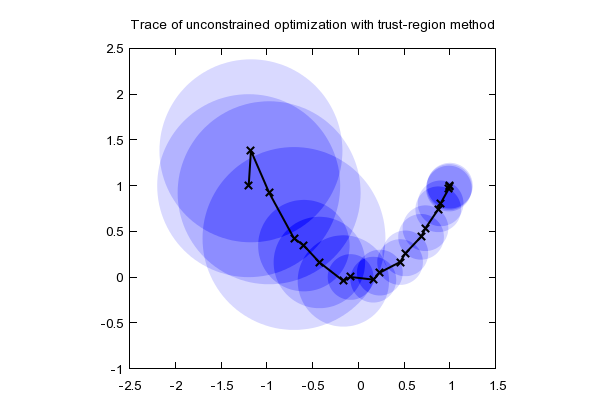
\includegraphics[width=0.6\textwidth]{img/TRM.png}
\end{figure}
\section{信赖域算法框架}
\begin{figure}[h!]
\caption{步长和改进方向都是预定信赖域大小的结果}
\centering
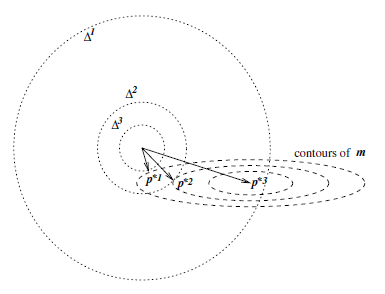
\includegraphics[width=0.6\textwidth]{img/TRM_stepsize.png}
\end{figure}
由带Lagrange余项的Taylor公式,有
\begin{equation*}
	f(x^k+d) = f(x^k) + \nabla f(x^k)^T d +\frac{1}{2}d^T\nabla^2 f(x^k+td)d,
\end{equation*}
其中$t\in (0, 1)$.我们用$f$的二阶近似来刻画$f(x)$在$x=x^k$的性质:
\begin{equation}\label{model_function}
	m_k(d) = f(x^k) +\nabla f(x^k)^Td + \frac{1}{2}d^TB^kd,
\end{equation}
$B^k$是对称矩阵,要求$B^k$是Hessian矩阵的近似.若$B^k$恰好是Hessian矩阵, 则$m_k(d)$的近似误差为$\mathcal{O}(||d||^3)$.\par
考虑到Taylor展开是函数的局部性质,于是我们仅在下面的求内考虑问题
\begin{equation*}
	\Omega_k = \{x^k + d\mid ||d||\leq \Delta_k\}
\end{equation*}
其中$\Delta_k$是一个与迭代有关的参数.我们称$\Omega_k$为\textbf{信赖域},$\Delta_k$为\textbf{信赖域步长}.我们相信在信赖域中$m_k(d)$能够很好地近似$f(x)$,因此信赖域算法每一步都要解决如下的子问题:
\begin{equation}\label{subp}
	\min\limits_{d\in \mathbb{R}^n} m_k(d),\quad s.t.\quad ||d||\leq \Delta_k.
\end{equation}
事实上,在信赖域算法中,选取信赖域半径至关重要,它决定了算法的收敛性.考虑到信赖域半径是“对模型函数$m_k(d)$相信的程度”,那么如果$m_k(d)$对函数$f(x)$近似较好,我们应扩大信赖域半径,反之就应该减小信赖域重新计算.我们引入如下的定义来衡量模型函数$m_k(d)$近似的好坏:
\begin{equation}\label{rho}
	\rho_k = \frac{f(x^k)-f(x^k+d)}{m_k(0)-m_k(d^k)},
\end{equation}
其中$d^k$为求解信赖域问题子问题\eqref{subp}得到的迭代方向.根据$\rho_k$的定义我们知道它即为函数值实际下降量与预估下降量的比值.如果$\rho_k$接近$1$,说明$m_k(d)$近似$f(x)$是比较成功的,我们应该扩大$\Delta_k$,否则应该缩小信赖域.
下面我们给出具体的算法,注意我们其实回避了如何求解子问题\eqref{subp}
\begin{algorithm}[H]
%\footnotesize%字体大小
\caption{信赖域算法}%首行显示算法名称
\begin{algorithmic}[1]%行编号,从Input, Output后面开始
%输入Input
\Require 最大半径$\Delta_max$,初始半径$\Delta_0$,初始点$x^0$,$k\leftarrow 0$.
\Require 给定参数$0\leq \eta < \bar{\rho_1}<\bar{\rho_2}<1$,$\gamma_1<1<\gamma_2$.

\While{未达到收敛准则}
\State 计算信赖域问题子问题\eqref{subp}得到迭代方向$d^k$(实际上是步长+方向).
\State 根据\eqref{rho}计算下降率$\rho_k$.
\If {$\rho < \bar\rho_1$}
	\State 缩小信赖域半径: $\Delta_{k+1}\leftarrow \gamma_1 \Delta_k$.
\Else
	\If{$\rho_k>\bar\rho_2$以及$||d^k||=\Delta_k$}
		\State 扩大信赖域半径:$\Delta_{k+1} \leftarrow \min\{\gamma_2\Delta_k, \Delta_{max}\}$.
	\Else
		\State 信赖域半径不变:$\Delta_{k+1}\leftarrow \Delta_k$	
	\EndIf
\EndIf
\If{$\rho_k> \eta$}
	\State 更新$x^{k+1} \leftarrow x^k+d^k$.
\Else
	\State $x^{k+1}\leftarrow x^k$.
\EndIf
\State $k\leftarrow k+1.$
\EndWhile
\end{algorithmic}  
\end{algorithm}
实际上,信赖域算法的大致思想就是首先判断模型函数$m_k(d)$是否是原函数$f(x)$在$\Delta_k$中的良好近似,并根据此修改信赖域半径.接着迈出步子走就好了.\par
我们通常取参数如下:$\bar\rho_1 = 0.25, \bar\rho_2=0.75$以及$\gamma_1=0.25, \gamma_2 = 2$.\par
下面我们给出求解信赖域子问题\eqref{subp}的算法.而这才是信赖域算法的关键.
\section{信赖域算法子问题求解}
信赖域子问题\eqref{subp}仅仅是一个涉及二次函数的约束优化问题,我们可以通过KKT条件求解,通过KKT条件得到最优解$d^*$应满足如下条件(过程太长, 详情参见文再文老师的书):
\begin{theorem}
	$d^*$是信赖域子问题
	\begin{equation*}
		\min\quad m(d) = f + g^Td+\frac{1}{2}d^TBd, \quad s.t.\quad ||d||\leq \Delta
	\end{equation*}
	的全局极小解当且仅当$d^*$可行且存在$\lambda\geq 0$满足
	\begin{equation}
		\begin{split}
			(B+\lambda I)d^* &= -g,\\
			\lambda(\Delta- ||d^*||) &= 0,\\
			(B+\lambda I)& \succeq 0.
		\end{split}
	\end{equation}
\end{theorem}
寻找子问题\eqref{subp}的近似解常有三种方法
\begin{enumerate}
	\item Cauchy点
	\item Dogleg算法(针对$B_k\succ 0$)
	\item 二维子空间极小化(对于$B_k$非正定)
\end{enumerate}
首先我们介绍Cauchy点
\subsection{Cauchy点}
\begin{definition}[Cauchy点]
	设$m_k(d)$是$f(x)$在点$x=x^k$处的二阶近似,常数$\tau_k$为如下优化问题的解
	\begin{equation*}
		\begin{split}
			&\min\quad m_k(-\tau \nabla f(x^k)),\\
			&s.t.\quad ||\tau \nabla f(x^k)||\leq \Delta_k, \tau\geq 0
		\end{split}
	\end{equation*}
	称$x_C^k\vcentcolon = x^k + d_C^k$为Cauchy点,其中$d_C^k = -\tau_k\nabla f(x^k)$.
\end{definition}
实际上,根据Cauchy点的定义, 它实际上是对$m_k(d)$进行一次精确线搜索的梯度法,只不过这个线搜索是考虑了信赖域约束的,参见下图
\begin{figure}[h!]
\caption{Cauchy点}
\centering
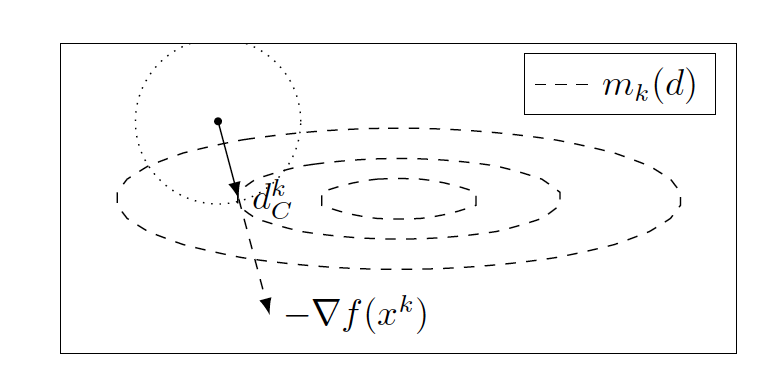
\includegraphics[width=0.6\textwidth]{img/cauchypoint.png}
\end{figure}
事实上, 根据定义,Cauchy点能够显式地计算出来,为方便起见,我们用$g^k$表示$\nabla f(x^k)$
\begin{equation*}
	\tau_k = \begin{cases}
		\frac{\Delta_k}{||g_k||}, & (g^k)^TB^kg^k\leq 0,\\
		\min\{\frac{||g^k||^2}{(g^k)^TB^kg^k},\frac{\Delta_k}{||g^k||}\}, &\text{其它}.
	\end{cases}
\end{equation*}
\subsection{dog leg 法}
Dog let法由Powell提出,结合了Gauss–Newton算法和梯度下降法,但是使用了显式信任区域。在每次迭代中,如果高斯-牛顿算法中的步骤位于信任区内,则将其用于更新当前解决方案。如果不是,则算法沿最陡的下降方向(称为柯西点)搜索目标函数的最小值。如果柯西点在信任区域之外,则将其截断到信任区域的边界,并将其作为新的解决方案。如果柯西点在信任区域内,则在信任区域边界与连接柯西点和Gauss-Newton步(dog leg step)的线之间的交点处采用新解。\par
\begin{note}
	我真的找不到太多dog leg法的资料, 它的slide味同嚼蜡看不懂.以后有心情再了解.
\end{note}
\clearpage
\pagestyle{numberonly}
\printbibliography

\end{document}
